\documentclass[./thesis.tex]{subfiles}

\begin{document}
\label{chap:PERF}

In this chapter, we discuss the efficiency of the implementation. The system
we chose for these numerical experiments is a cyanine dye, \\
\begin{center}
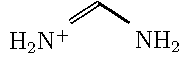
\includegraphics[]{figures/perf/Cyanine} \\
\end{center}
%[(NH$_2$)(CH)(NH$_2$)]$^+$
in its ground state and in its first excited state.
The geometry is the equilibrium geometry of the ground state, optimized at the
PBE0/cc-pVQZ level. The ground state is a closed shell, well described by a
single reference, and the excited state is singly excited and requires two
determinants in the reference ($1/\sqrt{2} (a\bar{b} + b\bar{a})$).  The
calculations were performed in the aug-cc-pVDZ basis set with state-averaged
natural orbitals obtained from an initial CIPSI calculation.
The $1s$ orbitals of the carbon and the nitrogen atoms were frozen, so
the FCI space which is explored is a CAS(18,111). The reference excitation
energy, obtained at the CC3/ANO-L-VQZP level is 7.18~eV.\cite{Send_2011}
The measurements were made on the Olympe supercomputer (CALMIP). Each node is 
a dual-socket Intel(R) Xeon(R) Gold 6140 CPU @ 2.30GHz with 192GiB of RAM, and
contains 36 physical CPU cores. Parallel speedup curves are made with up to
$1~800$~cores for the four main parts presented in this manuscript, namely the
Davidson diagonalization, the CIPSI selection, the hybrid
stochastic/deterministic computation of $\EPT$ and the matrix dressing.

\begin{figure}[hbt]
	\begin{center}
		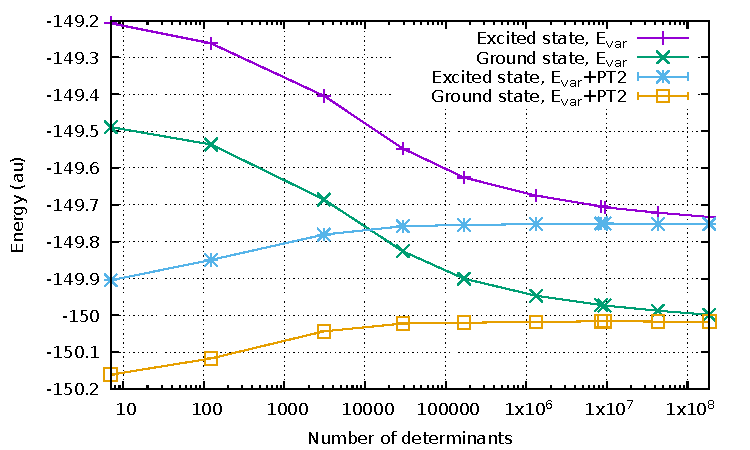
\includegraphics[width=0.8\columnwidth]{figures/perf/cn3_energy}
		\caption{Convergence of the energy of the ground and excited states with respect to the number of determinants in the variational space.}
		\label{fig:energy_pt2}
	\end{center}
\end{figure}

\begin{table}[hbt]
\caption{Energies and second-order perturbative corrections for increasingly large wavefunctions. $\Delta E$ is the energy difference
between the ground state and the excited state.}
\label{tab:energy_pt2}
\begin{center}
\begin{tabular}{rllrr}
\hline
\tabc{$\Ndet$} & \tabc{Ground state} & \tabc{Excited state} & \tabc{$\Delta E$ (eV)} \\
\hline
\multicolumn{4}{c}{$\Evar$}  \\
$          7$ & $-149.489~186$ & $-149.207~354$ & $7.67$  \\
$        123$ & $-149.536~265$ & $-149.261~860$ & $7.47$  \\
$      3~083$ & $-149.685~606$ & $-149.404~450$ & $7.65$  \\
$     29~409$ & $-149.826~151$ & $-149.547~275$ & $7.59$  \\
$    168~595$ & $-149.900~352$ & $-149.626~058$ & $7.46$  \\
$  1~322~537$ & $-149.946~655$ & $-149.675~032$ & $7.39$  \\
$  8~495~334$ & $-149.972~032$ & $-149.704~145$ & $7.29$  \\
$  9~356~952$ & $-149.973~375$ & $-149.706~822$ & $7.25$  \\
$ 42~779~636$ & $-149.987~370$ & $-149.721~470$ & $7.24$  \\
$186~978~487$ & $-149.998~582$ & $-149.733~039$ & $7.23$  \\
\hline

\multicolumn{4}{c}{$\Evar + \EPT$}  \\
$          7$ & $-150.161~107  $ & $-149.904~883  $ & $6.97$ \\
$        123$ & $-150.116~958  $ & $-149.849~465  $ & $7.28$ \\
$      3~083$ & $-150.043~5(2) $ & $-149.780~8(2) $ & $7.15$ \\
$     29~409$ & $-150.022~2(2) $ & $-149.758~3(2) $ & $7.18$ \\
$    168~595$ & $-150.019~9(1) $ & $-149.754~5(1) $ & $7.22$ \\
$  1~322~537$ & $-150.017~89(7)$ & $-149.752~55(7)$ & $7.22$ \\
$  8~495~334$ & $-150.015~97(4)$ & $-149.750~87(5)$ & $7.21$ \\
$  9~356~952$ & $-150.015~89(3)$ & $-149.750~66(3)$ & $7.22$ \\
$ 42~959~496$ & $-150.016~75(2)$ & $-149.751~88(2)$ & $7.21$ \\
$186~978~487$ & $-150.017~51(2)$ & $-149.752~90(2)$ & $7.20$ \\
\hline
\end{tabular}
\end{center}
\end{table}

In figure~\ref{fig:energy_pt2}, we plot the convergence of the energies of
the ground and excited states as a function of the number of
determinants, with and without the second order perturbative contribution.
From these data, one can see that although $\EPT$ is still large ($\sim 0.02$~au)
the excitation energies both at the variational level and with the perturbative
correction converge to a value of $7.20$~eV compatible with the reference
energy obtained in a larger basis set.



\clearpage

\section{Davidson diagonalization}


First, we measure the time required to compute one iteration of the Davidson algorithm with increasingly large wave functions. The results are reported in table~\ref{tab:time_davidson_ndet}.

\begin{table}[hbt]
\caption{Wall-clock time (in seconds) to run one Davidson's iteration in parallel with increasingly large wavefunctions.}
\label{tab:time_davidson_ndet}
\begin{center}
\begin{tabular}{rr}
\hline
\tabc{$\Ndet$} & \tabc{seconds} \\
\hline
$    29~409$ &       $2.72$ \\
$   168~595$ &       $4.21$ \\
$ 1~322~537$ &      $56.24$ \\
$ 9~356~952$ &     $775.55$ \\
$42~959~496$ &  $11~198.70$ \\
\hline
\end{tabular}
\end{center}
\end{table}

\begin{figure}[h]
    \begin{center}
      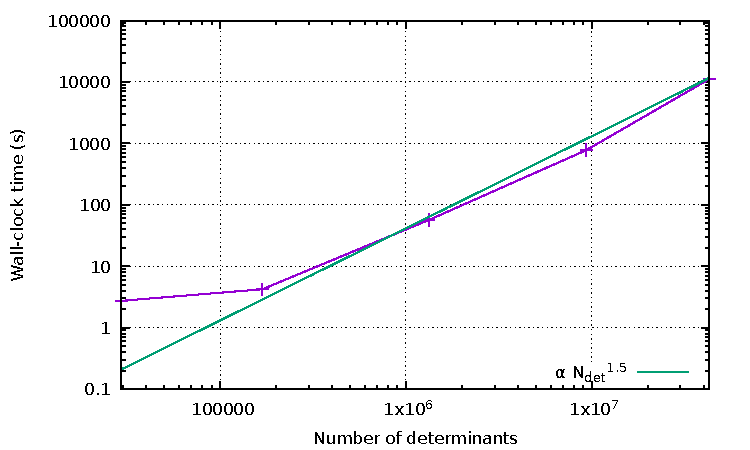
\includegraphics[width=0.8\columnwidth]{figures/perf/scaling_davidson_ndet}
      \caption{Wall-clock time of one Davidson iteration as a function of the number of
determinants in the wavefunction.}
      \label{fig:speedup_davidson_ndet}
    \end{center}
\end{figure}

Plotting this data with a log-log scale (figure~\ref{fig:speedup_davidson_ndet}) shows an agreement with the predicted $\order{\Ndet^{3/2}}$ scaling.

Then, we took the two largest wavefunctions. One with $9~356~952$ and one with $42~959~496$ determinants, and measured the wall-clock time required to
perform one iteration of the Davidson diagonalization, with an increasing number of compute nodes.

\begin{table}[hbt]
\caption{Wall-clock time (in seconds) to run one Davidson's iteration in parallel on two different wavefunctions 
with an increasing number of 36-core compute nodes.}
\label{tab:time_davidson}
\begin{center}
\begin{tabular}{rrr}
\hline
\tabc{Nodes} & \tabc{9~356~952 determinants} & \tabc{42~959~496 determinants} \\
\hline
$ 1$ &$775.55$ &$11~198.70$\\
$ 5$ &$169.88$ &$ 2~288.58$\\
$10$ &$ 93.22$ &$ 1~213.95$\\
$20$ &$ 56.86$ &$   626.41$\\
$30$ &$ 43.76$ &$   445.65$\\
$40$ &$ 36.18$ &$   350.25$\\
$50$ &$ 33.67$ &$   295.25$\\
\hline
\end{tabular}
\end{center}
\end{table}

\begin{figure}[h]
    \begin{center}
      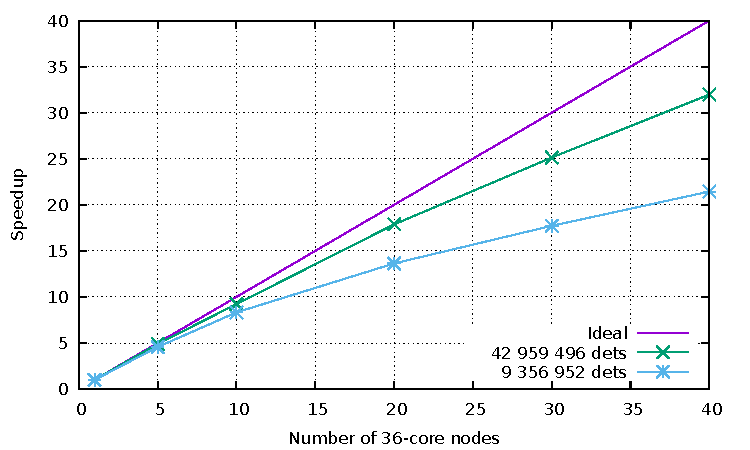
\includegraphics[width=0.8\columnwidth]{figures/perf/scaling_davidson}
      \caption{Speedup of one Davidson iteration as a function of the number of
36-core compute nodes.}
      \label{fig:speedup_davidson}
    \end{center}
\end{figure}

The timings are reported in table~\ref{tab:time_davidson} and the parallel speedup curve is represented in figure~\ref{fig:speedup_davidson}. Using a log-log plot, we were able to fit the data and find
a scaling as $\order{\Ndet^{3/2}}$, as expected.  As the communication scales as $\order{\Ndet}$, 
the parallel efficiency increases together with $\Ndet$, as shown on figure~\ref{fig:speedup_davidson}.


\clearpage

\section{Selection}

\begin{table}[hbt]
\caption{Single-node (36-core) CIPSI selection for increasingly large wavefunctions. Time is given in seconds.}
\label{tab:time_selection}
\begin{center}
\begin{tabular}{rr}
\hline
\tabc{$\Ndet$} & \tabc{seconds} \\
\hline
$      123$ & $      0.14$ \\
$    3~083$ & $      0.59$ \\
$   29~409$ & $     42.67$ \\
$  168~595$ & $    239.21$ \\
$1~322~537$ & $  2~008.76$ \\
$9~356~952$ & $ 22~560.33$ \\
\hline
\end{tabular}
\end{center}
\end{table}

\begin{table}[hbt]
\caption{Time (in seconds) to run parallel CIPSI selections on the
9~356~952-determinant wavefunction with an increasing number of 36-core
compute nodes.}
\label{tab:selection_parallel}
\begin{center}
\begin{tabular}{rr}
\hline
\tabc{Nodes} & \tabc{seconds}  \\
\hline
$ 1$ & $22~560.33$ \\
$ 5$ & $ 4~468.28$ \\
$10$ & $ 2~245.00$ \\
$20$ & $ 1~137.67$ \\
$30$ & $   769.58$ \\
$40$ & $   582.62$ \\
$50$ & $   472.33$ \\
\hline
\end{tabular}
\end{center}
\end{table}

\begin{figure}[hbt]
    \begin{center}
      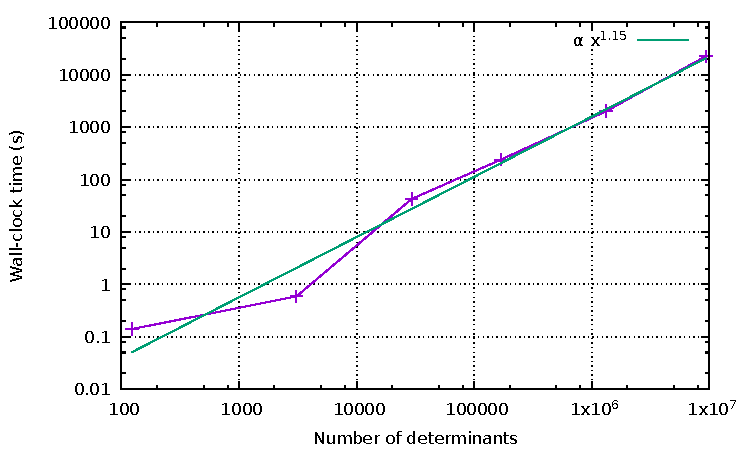
\includegraphics[width=0.8\columnwidth]{figures/perf/scaling_sel_det}
      \caption{Wall-clock time of the selection as a function of the number of
determinants in the wavefunction.}
      \label{fig:scaling_sel_ndet}
    \end{center}
\end{figure}

\begin{figure}[h]
    \begin{center}
      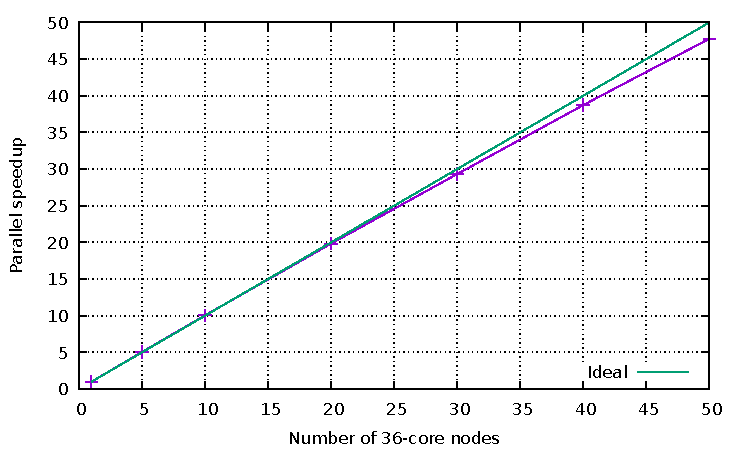
\includegraphics[width=0.8\columnwidth]{figures/perf/scaling_sel_node}
      \caption{Parallel speedup of the CIPSI selection. The reference is a single 36-core node.}
      \label{fig:speedup_sel_node}
    \end{center}
\end{figure}

We have measured the time necessary to realize a selection step, with an
increasing number of determinants in the variational space.
Figure~\ref{fig:scaling_sel_node} shows a near-linear scaling with the number of
determinants. This is due to the threshold $n_g$ which tends to make the number of external determinants constant when the wavefunction becomes large enough.

The parallel speedup was also measured with up to 50 nodes, showing an almost ideal speedup curve. This is in part due to the tuning of the fragmentation of the
tasks which gives a very well balanced task queue.

\clearpage

\section{PT2 calculations}

The algorithms for the computation $\EPT$ are very similar to those of the CIPSI selection. Therefore, we expect a similar behavior with $\Ndet$ and with the number of nodes.

The stopping criterion of the calculation of the $\EPT$ contribution was a
relative statistical error below 1/1000-th. Hence, the error bar decreases with
the number of determinants, but the fraction of the full deterministic
calculation required to reach this criterion is relatively stable around $5$\%.

\begin{figure}[hbt]
	\begin{center}
		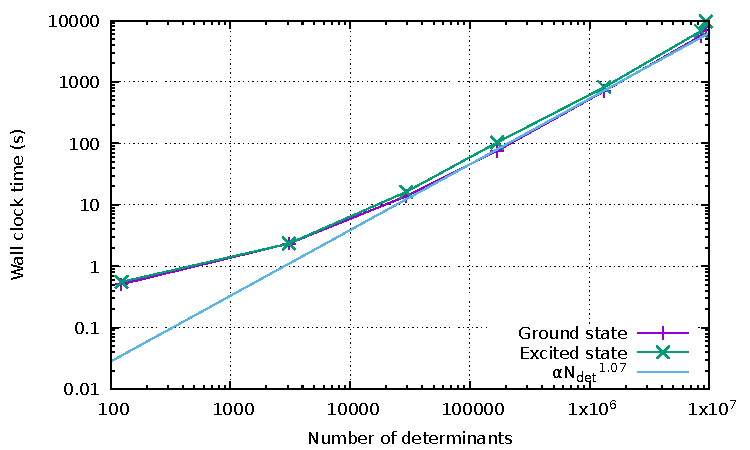
\includegraphics[width=0.8\columnwidth]{figures/perf/scaling_pt2_det}
		\caption{Wall clock time required to compute $\EPT$ for the ground and the excited states, as a function of the number of determinants in the wavefunction.}
		\label{fig:scaling_det_pt2}
	\end{center}
\end{figure}

\begin{table}[hbt]
\caption{Single-node (36-core) $\EPT$ calculations for increasingly large wavefunctions. Time is given in seconds.}
\label{tab:time_pt2}
\begin{center}
\begin{tabular}{rrr}
\hline
\tabc{$\Ndet$} & \tabc{Ground state} & \tabc{Excited state} \\
\hline
$      123$ &  $     0.51$ & $     0.56$ \\
$    3~083$ &  $     2.33$ & $     2.34$ \\
$   29~409$ &  $    13.83$ & $    16.21$ \\
$  168~595$ &  $    75.62$ & $   103.26$ \\
$1~322~537$ &  $   708.53$ & $   818.58$ \\
$8~495~334$ &  $ 5~578.76$ & $ 6~751.25$ \\
$9~356~952$ &  $ 7~779.80$ & $ 9~663.79$ \\
\hline
\end{tabular}
\end{center}
\end{table}

Table~\ref{tab:time_pt2} reports the wall-clock time required to compute $\EPT$
on a single node.
From these data, one can evaluate the scaling of the cost of $\EPT$ 
with the number of determinants, as plotted in figure~\ref{fig:scaling_det_pt2},
which is close to linear.
This can be understood, since 
the number of $\ket{\alpha}$ determinants is proportional to the
number of determinants in the variational wavefunction, and each
$\ket{\alpha}$ needs to be compared to all the determinants 
in the computation of $\mel{\alpha}{H}{\Psi}$.
But when the wavefunction becomes large enough, the second point is not true any more because only a limited number of determinants $\ket{I}$ of $\Psi$ have a non-zero
value $\mel{\alpha}{H}{I}$, and this number is bounded by the number of single and double excitations, characteristic of the basis set.
Fitting the last points with a log-log plot shows an asymptotic scaling as
$\order{\Ndet^{1.07}}$, which is expected to be linear for very large numbers 
of determinants.

\begin{table}
\caption{Time (in seconds) to run parallel $\EPT$ calculations on the largest wavefunction with an
increasing number of 36-core compute nodes.}
\label{tab:pt2_parallel}
\begin{center}
\begin{tabular}{rrr}
\hline
\tabc{Nodes} & \tabc{Ground state} & \tabc{Excited state} \\
\hline
$1 $ & $7~779.80$  & $9~663.79$  \\ %TODO
$5 $ & $1~649.26$  & $2~037.44$  \\
$10$ & $  854.52$  & $1~054.09$  \\
$20$ & $  461.96$  & $  560.73$  \\
$30$ & $  352.26$  & $  424.19$  \\
$40$ & $  281.51$  & $  331.23$  \\
$50$ & $  225.08$  & $  278.21$  \\
\hline
\end{tabular}
\end{center}
\end{table}
\begin{figure}[hbt]
	\begin{center}
		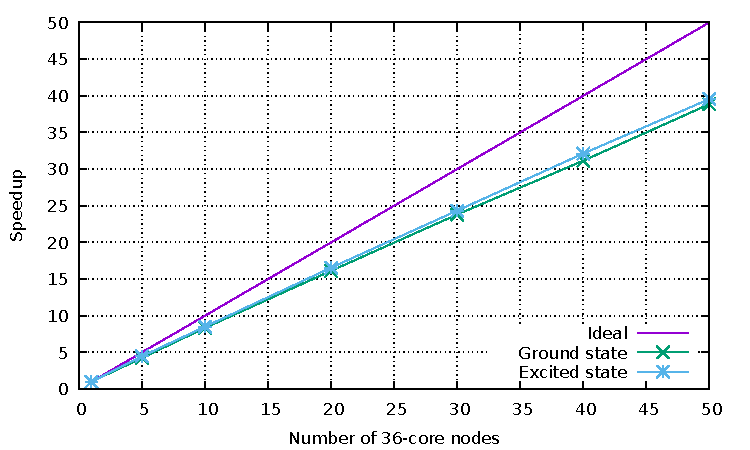
\includegraphics[width=0.8\columnwidth]{figures/perf/scaling_pt2_node}
		\caption{Parallel speedup for the calculation of the $\EPT$ contribution of the ground state using the largest wavefunction. Each node contains 36 physical CPU cores.}
		\label{fig:scaling_node_pt2}
	\end{center}
\end{figure}

To analyze the parallel efficiency of the $\EPT$ calculation, we have made the parallel speedup curve using up to 50 nodes (1800 CPU cores), plotted in figure~\ref{fig:scaling_node_pt2}. With 50 nodes, one obtains a speedup with respect to the single-node reference of $35\times$ for both the ground and excited states. This corresponds to a parallel efficiency of 70\%, which is less satisfactory than the almost ideal speedup obtained for the selection.

There are two reasons for this disappointing speedup. The first one is that the calculation is aborted when the target precision is below a given threshold. So when more compute nodes are used, more samples are gathered at the end of the calculation and the computation is more precise. In the limit of $\Ndet$ CPU cores, only the deterministic calculation can be done, whatever the stopping criterion. So the computation of the speedup is not 100\% fair.
The second reason for the on-ideal speedup is the pre-computation of the combs on the master process which delays the start of the computation of the tasks.

\clearpage

\section{Matrix dressing}

The algorithms for the matrix dressing are similar to those of $\EPT$. Therefore, we expect a similar behavior with $\Ndet$ and with the number of nodes.

\begin{table}[hbt]
\caption{Single-node (36-core) Shifted-$B_k$ iteration for increasingly large wavefunctions.
Time is given in seconds.}
\label{tab:time_selection}
\begin{center}
\begin{tabular}{rrr}
\hline
\tabc{$\Ndet$} & \tabc{Ground state} & \tabc{Excited state} \\
\hline
$      123$ & $      0.80$  & $      0.78$ \\
$    3~083$ & $      4.06$  & $      5.38$ \\
$   29~409$ & $     27.27$  & $     29.45$ \\
$  168~595$ & $    129.93$  & $    201.65$ \\
$1~322~537$ & $  1~518.60$  & $  1~766.36$ \\
$9~356~952$ & $ 15~004.54$  & $ 17~766.99$ \\
\hline
\end{tabular}
\end{center}
\end{table}
\begin{figure}[hbt]
	\begin{center}
		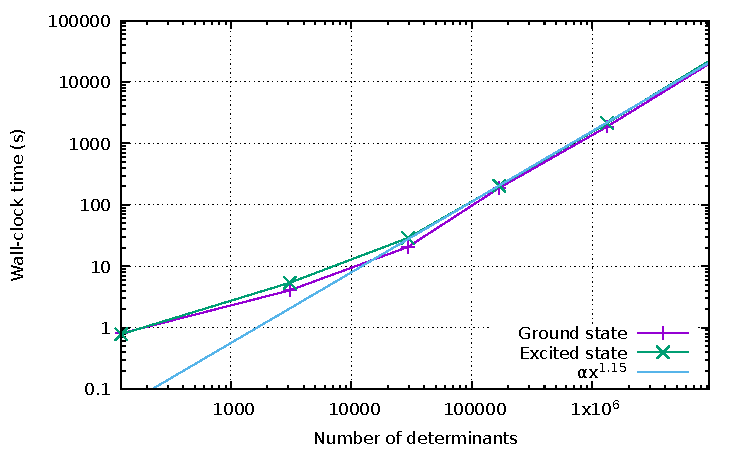
\includegraphics[width=0.8\columnwidth]{figures/perf/scaling_sbk_det}
		\caption{Wall clock time required to compute the Shifted-$B_k$ dressing for the ground and the excited states, as a function of the number of determinants in the wavefunction.}
		\label{fig:scaling_det_sbk}
	\end{center}
\end{figure}

The time necessary to build the dressing matrix in the Shifted-$B_k$ method was measured on a single
36-core node with an increasing number of determinants (figure~\ref{fig:scaling_det_sbk}).
As for $\EPT$, the stopping criterion was an estimated relative error on 
$\mel{\Psi}{\hat \Delta}{\Psi}$, the dressed energy, equal to $0.001$.

Using the log-log plot, the scaling with the number of determinants was found to be
$\order{\Ndet^{1.15}}$.
This scaling is slightly higher than the $\order{\Ndet^{1.07}}$ measured for $\EPT$,
but close to linear, as expected. The additional overhead is due to the handling of
the checkpoints which eliminates the communication bottleneck.

\begin{center}
\begin{tabular}{rrr}
\hline
\tabc{Nodes} & \tabc{Ground state} & \tabc{Excited state} \\
\hline
$1 $ & $7~779.80$  & $9~663.79$  \\ %TODO
$5 $ & $1~649.26$  & $2~037.44$  \\
$10$ & $  854.52$  & $1~054.09$  \\
$20$ & $  461.96$  & $  560.73$  \\
$40$ & $  281.51$  & $  331.23$  \\
$50$ & $  225.08$  & $  278.21$  \\
\hline
\end{tabular}
\end{center}
\begin{figure}[hbt]
	\begin{center}
		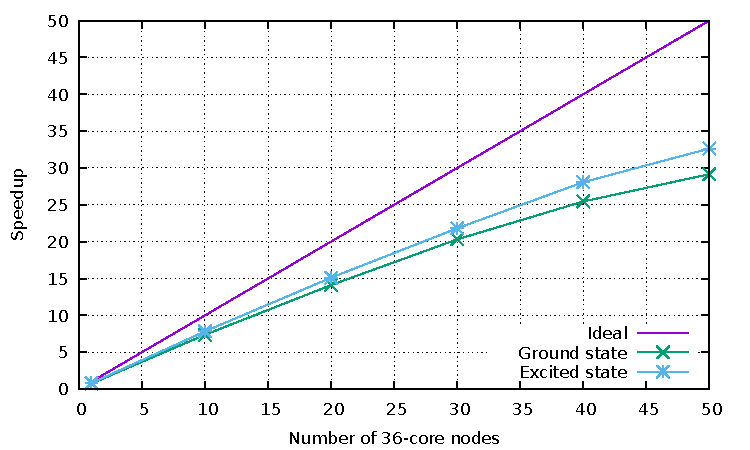
\includegraphics[width=0.8\columnwidth]{figures/perf/scaling_sbk_node}
		\caption{Parallel speedup for the calculation of the matrix dressing of the ground state using the largest wavefunction. Each node contains 36 physical CPU cores.}
		\label{fig:scaling_node_sbk}
	\end{center}
\end{figure}

Then, the parallel speedup was measured using the wavefunction with 9~356~952 determinants. The results
are plotted in figure~\ref{fig:scaling_node_sbk}.

\clearpage

\end{document}
